\def\epsx{.12}
\newcommand{\vertexoo}[1]{\scalebox{#1}{\begin{tikzpicture}
[scale=1, very thick]
\node (i1) at (0,-1) {$g$};
\node (j1) at (-1,0) {$0$};
\node (i2) at (0,1) {$g$};
\node (j2) at (1,0) {$0$};
% \draw (i1) -- (i2);
\draw[densely dotted] (j1) -- (j2);
% \draw[densely dotted] (i1) -- (i2);
\foreach \shi in {(0,0), (\epsx,0), (-\epsx,0)}
{\begin{scope}[shift=\shi]
\node (shi1) at (0,-1) {\phantom{$g$}};
\node (shi2) at (0,1) {\phantom{$g$}};
\draw[->] (shi1) -- (shi2);
\draw[->] (shi1) --++ (0,.5);
% \draw[->] (0,\epsx) -- (shi2);
\end{scope}}
% \draw[fill] (0,0) circle (3pt);
\end{tikzpicture}}}
\newcommand{\vertexol}[1]{\scalebox{#1}{\begin{tikzpicture}
[scale=1, very thick]
\node (i1) at (0,-1) {$g$};
\node (j1) at (-1,0) {$0$};
\node (i2) at (0,1) {$g-1$};
\node (j2) at (1,0) {$1$};
\foreach \shi in {(0,0), (-\epsx,0)}
{\begin{scope}[shift=\shi]
\node (shi1) at (0,-1) {\phantom{$g$}};
\node (shi2) at (0,1) {\phantom{$g$}};
\draw[->] (shi1) -- (shi2);
\draw[->] (shi1) --++ (0,.5);
% \draw[->] (0,\epsx) -- (shi2);
\end{scope}}
% \draw[fill] (0,0) circle (3pt);
\foreach \shi in {(\epsx,0)}
{\begin{scope}[shift=\shi]
\node (shi1) at (0,-1) {\phantom{$g$}};
\node (shi2) at (0,1) {\phantom{$g$}};
\draw[->] (shi1) -- (0,0) -- (j2);
\draw[->] (shi1) --++ (0,.5);
% \draw[->] (0,0) -- (shi2);
\end{scope}}
\draw[densely dotted] (j1) -- (j2);
% \draw[->] (\epsx,0) -- (j2);
\end{tikzpicture}}}

\newcommand{\vertexoll}[1]{\scalebox{#1}{\begin{tikzpicture}
[scale=1, very thick]
\node (i1) at (0,-1) {$g+1$};
\node (j1) at (-1,0) {$0$};
\node (i2) at (0,1) {$g$};
\node (j2) at (1,0) {$1$};
\foreach \shi in {(-1.5*\epsx,0), (.5*\epsx,0),(-.5*\epsx,0)}
{\begin{scope}[shift=\shi]
\node (shi1) at (0,-1) {\phantom{$g$}};
\node (shi2) at (0,1) {\phantom{$g$}};
\draw[->] (shi1) -- (shi2);
\draw[->] (shi1) --++ (0,.5);
% \draw[->] (0,\epsx) -- (shi2);
\end{scope}}
% \draw[fill] (0,0) circle (3pt);
\foreach \shi in {(1.5*\epsx,0)}
{\begin{scope}[shift=\shi]
\node (shi1) at (0,-1) {\phantom{$g$}};
\node (shi2) at (0,1) {\phantom{$g$}};
\draw[->] (shi1) -- (0,0) -- (j2);
\draw[->] (shi1) --++ (0,.5);
% \draw[->] (0,0) -- (shi2);
\end{scope}}
\draw[densely dotted] (j1) -- (j2);
% \draw[->] (\epsx,0) -- (j2);
\end{tikzpicture}}}

\newcommand{\vertexll}[1]{\scalebox{#1}{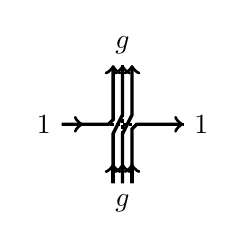
\begin{tikzpicture}
[scale=1, very thick]
% \draw[fill] (0,0) circle (3pt);
\node (i1) at (0,-1) {$g$};
\node (i1shm1) at (-\epsx,-1) {\phantom{$g$}};
\node (i1sh1) at (\epsx,-1) {\phantom{$g$}};
\node (j1) at (-1,0) {$1$};
\node (i2) at (0,1) {$g$};
\node (i2shm1) at (-\epsx,1) {\phantom{$g$}};
\node (i2sh1) at (\epsx,1) {\phantom{$g$}};
\node (j2) at (1,0) {$1$};
\draw[densely dotted] (j1) -- (j2);
\draw[densely dotted] (i1) -- (i2);
\draw[->] (j1) -- (-\epsx*1.5,0)--++(.5*\epsx,.5*\epsx) -- (i2shm1);
\draw[->] (i1shm1) -- (-\epsx,-\epsx) -- (0,\epsx) -- (i2);
\draw[->] (i1) -- (0,-\epsx) -- (\epsx,\epsx) -- (i2sh1);
\draw[->] (i1sh1) -- (\epsx,-.5*\epsx)--++(.5*\epsx,.5*\epsx) -- (j2);
\draw[->] (j1) --++ (.5,0);
\draw[->] (i1) --++ (0,.5);
\draw[->] (i1sh1) --++ (0,.5);
\draw[->] (i1shm1) --++ (0,.5);
\end{tikzpicture}}}
\newcommand{\vertexlo}[1]{\scalebox{#1}{\begin{tikzpicture}
[scale=1, very thick]
\node (i1) at (0,-1) {$g$};
\node (j1) at (-1,0) {$1$};
\node (i2) at (0,1) {$g+1$};
\node (i2shm2) at (-3/2*\epsx,1) {\phantom{$g$}};
\node (j2) at (1,0) {$0$};
\draw[densely dotted] (j1) -- (j2);
\draw[->] (j1) -- (-3/2*\epsx,0) -- (i2shm2);
\foreach \shi in {(1/2*\epsx,0), (3/2*\epsx,0), (-1/2*\epsx,0)}
{\begin{scope}[shift=\shi]
\node (shi1) at (0,-1) {\phantom{$g$}};
\node (shi2) at (0,1) {\phantom{$g$}};
\draw[->] (shi1) -- (shi2);
\draw[->] (shi1) --++ (0,.5);
\end{scope}}
\draw[->] (j1) --++ (.5,0);
% \draw[fill] (0,0) circle (3pt);
\end{tikzpicture}}}







\newcommand{\Bvertexoo}[1]{\scalebox{#1}{\begin{tikzpicture}
[scale=1, very thick]
\node (i1) at (0,-1) {$g$};
\node (j1) at (-1,0) {$0$};
\node (i2) at (0,1) {$g$};
\node (j2) at (1,0) {$0$};
\draw[densely dotted] (j1) -- (j2);
\foreach \shi in {(0,0), (\epsx,0), (-\epsx,0)}
{\begin{scope}[shift=\shi]
\node (shi1) at (0,1) {\phantom{$g$}};
\node (shi2) at (0,-1) {\phantom{$g$}};
\draw[->] (shi1) -- (shi2);
\draw[->] (shi1) --++ (0,-.5);
% \draw[->] (0,\epsx) -- (shi2);
\end{scope}}
% \draw[fill] (0,0) circle (3pt);
\end{tikzpicture}}}

\newcommand{\Bvertexll}[1]{\scalebox{#1}{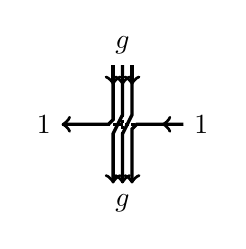
\begin{tikzpicture}
[scale=1, very thick]
\node (i1) at (0,1) {$g$};
\node (i1shm1) at (\epsx,1) {\phantom{$g$}};
\node (i1sh1) at (-\epsx,1) {\phantom{$g$}};
\node (j1) at (1,0) {$1$};
\node (i2) at (0,-1) {$g$};
\node (i2shm1) at (\epsx,-1) {\phantom{$g$}};
\node (i2sh1) at (-\epsx,-1) {\phantom{$g$}};
\node (j2) at (-1,0) {$1$};
\draw[densely dotted] (j1) -- (j2);
\draw[densely dotted] (i1) -- (i2);
\draw[->] (j1) -- (\epsx*1.5,0)--++(-.5*\epsx,-.5*\epsx) -- (i2shm1);
\draw[->] (i1shm1) -- (\epsx,\epsx) -- (0,-\epsx) -- (i2);
\draw[->] (i1) -- (0,\epsx) -- (-\epsx,-\epsx) -- (i2sh1);
\draw[->] (i1sh1) -- (-\epsx,.5*\epsx)--++(-.5*\epsx,-.5*\epsx) -- (j2);
\draw[->] (j1) --++ (-.5,0);
\draw[->] (i1) --++ (0,-.5);
\draw[->] (i1sh1) --++ (0,-.5);
\draw[->] (i1shm1) --++ (0,-.5);
\end{tikzpicture}}}

\newcommand{\Bvertexol}[1]{\scalebox{#1}{\begin{tikzpicture}
[scale=1, very thick]
\node (i1) at (0,1) {$g$};
\node (j1) at (1,0) {$0$};
\node (i2) at (0,-1) {$g-1$};
\node (j2) at (-1,0) {$1$};
\foreach \shi in {(0,0), (\epsx,0)}
{\begin{scope}[shift=\shi]
\node (shi1) at (0,1) {\phantom{$g$}};
\node (shi2) at (0,-1) {\phantom{$g$}};
\draw[->] (shi1) -- (shi2);
\draw[->] (shi1) --++ (0,-.5);
\end{scope}}
\foreach \shi in {(-\epsx,0)}
{\begin{scope}[shift=\shi]
\node (shi1) at (0,1) {\phantom{$g$}};
\node (shi2) at (0,-1) {\phantom{$g$}};
\draw[->] (shi1) -- (0,0) -- (j2);
\draw[->] (shi1) --++ (0,-.5);
\end{scope}}
\draw[densely dotted] (j1) -- (j2);
\end{tikzpicture}}}
\newcommand{\Bvertexlo}[1]{\scalebox{#1}{\begin{tikzpicture}
[scale=1, very thick]
\node (i1) at (0,1) {$g$};
\node (j1) at (1,0) {$1$};
\node (i2) at (0,-1) {$g+1$};
\node (i2shm2) at (3/2*\epsx,-1) {\phantom{$g$}};
\node (j2) at (-1,0) {$0$};
\draw[densely dotted] (j1) -- (j2);
\draw[->] (j1) -- (3/2*\epsx,0) -- (i2shm2);
\foreach \shi in {(-1/2*\epsx,0), (-3/2*\epsx,0), (1/2*\epsx,0)}
{\begin{scope}[shift=\shi]
\node (shi1) at (0,1) {\phantom{$g$}};
\node (shi2) at (0,-1) {\phantom{$g$}};
\draw[->] (shi1) -- (shi2);
\draw[->] (shi1) --++ (0,-.5);
\end{scope}}
\draw[->] (j1) --++ (-.5,0);
\end{tikzpicture}}}

